%%%%%%%%%%%%%%%%%%%%%%%%%%%%%%%%%%%%%%%%%%%%%%%%%%%%%%%%%%%%%%%%%%%%%%
%%                     Or
%%%%%%%%%%%%%%%%%%%%%%%%%%%%%%%%%%%%%%%%%%%%%%%%%%%%%%%%%%%%%%%%%%%%%%
\subsection{Glyph: \glyph{Or}}\label{sec:or}

The glyph \glyph{or} is used to denote that any of the \glyph{EPNs} linked as input is sufficient to produce the output. \glyph{Or} is represented by a circle carrying the word ``OR''.

\begin{figure}[H]
  \centering
  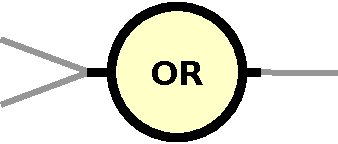
\includegraphics[scale = 0.5]{images/or}
  \caption{The \PD glyph for \glyph{or}. Only two inputs are represented, but more would be allowed.}
  \label{fig:or}
\end{figure}


